\let\negmedspace\undefined
\let\negthickspace\undefined
\documentclass[article]{IEEEtran}
\usepackage[a5paper, margin=10mm, onecolumn]{geometry}
%\usepackage{lmodern} % Ensure lmodern is loaded for pdflatex
\usepackage{tfrupee} % Include tfrupee package

\setlength{\headheight}{1cm} % Set the height of the header box
\setlength{\headsep}{0mm}     % Set the distance between the header box and the top of the text

\usepackage{gvv-book}
\usepackage{gvv}
\usepackage{cite}
\usepackage{amsmath,amssymb,amsfonts,amsthm}
\usepackage{algorithmic}
\usepackage{graphicx}
\usepackage{textcomp}
\usepackage{xcolor}
\usepackage{txfonts}
\usepackage{listings}
\usepackage{enumitem}
\usepackage{mathtools}
\usepackage{gensymb}
\usepackage{comment}
\usepackage[breaklinks=true]{hyperref}
\usepackage{tkz-euclide} 
\usepackage{listings}                                       
\def\inputGnumericTable{}                                 
\usepackage[latin1]{inputenc}                                
\usepackage{color}                                            
\usepackage{array}                                            
\usepackage{longtable}                                       
\usepackage{calc}                                             
\usepackage{multirow}                                         
\usepackage{hhline}                                           
\usepackage{ifthen}                                           
\usepackage{lscape}

\renewcommand{\thefigure}{\theenumi}
\renewcommand{\thetable}{\theenumi}
\setlength{\intextsep}{10pt} % Space between text and floats

\numberwithin{figure}{enumi}
\renewcommand{\thetable}{\theenumi}

% Marks the beginning of the document
\begin{document}
\bibliographystyle{IEEEtran}
\title{NCERT-10.4.ex.15}
\author{EE24BTECH11039 - MANDALA RANJITH}
{\let\newpage\relax\maketitle}


\subsection*{Question}
A motor boat whose speed is 18 km/h in still water takes 1 hour more to go 24 km upstream than to return downstream to the same spot. Find the speed of the stream.

\subsection*{Theoritical Solution}

Let the speed of the stream be  $x$  km/h.

Therefore, the speed of the boat upstream = $ \brak{18 - x}$ km/h and the speed of the boat downstream = $\brak{18 + x}$ km/h.

The time taken to go upstream is:
\begin{align}
\text{Time} = \frac{\text{Distance}}{\text{Speed}} = \frac{24}{18 - x} \text{ hours.}
\end{align}

Similarly, the time taken to go downstream is:
\begin{align}
\frac{24}{18 + x} \text{ hours.}
\end{align}

According to the question,
\begin{align}
\frac{24}{18 - x} - \frac{24}{18 + x} = 1
\end{align}

Multiplying throughout by \( 24(18 + x)(18 - x) \), we get:

\begin{align}
24(18 + x) - 24(18 - x) = (18 - x)(18 + x)
\end{align}

\begin{align}
x^2 + 48x - 324 = 0
\end{align}

Using the quadratic formula:

\begin{align}
x = \frac{-48 \pm \sqrt{48^2 + 1296}}{2} = \frac{-48 \pm \sqrt{3600}}{2}
\end{align}

\begin{align}
= \frac{-48 \pm 60}{2}
\end{align}

\begin{align}
= 6 \text{ or } -54
\end{align}
Since \( x \) is the speed of the stream, it cannot be negative. So, we ignore the root \( x = -54 \). 

Therefore, \( x = 6 \) gives the speed of the stream as \textbf{6 km/h}.

\begin{align}
    \textbf{Theorem: }
\end{align}
    Let $x = s$ be a solution of $x = g\brak{x}$ and suppose that $g$ has a continuous
    derivative in some interval $J$ containing $s$. Then if $\abs{g^{\prime}} \le K < 1$ in $J$,
    the iteration process defined  above converges for any $x_0$ in $J$. The limit of the sequence
    $\sbrak{x_n}$ is s\\
\newline
Since there is no solution (evident by quadratic formula) there exists no interval J for which
the process converges to a point.\\
\newline
The same behaviour is shown by the Newton-Raphson Method,\\
Start with an initial guess $x_0$, and then run the following logical loop,
\begin{align}
    x_{n+1} = x_n - \frac{f\brak{x_n}}{f^{\prime}\brak{x_n}} 
\end{align}
where ,
\begin{align}
    f\brak{x} = x^2 + 48x - 324\\
    f^{\prime}\brak{x} = 2x+48
\end{align}




\section*{Solving Using a Matrix Numerical Method (Fixed-Point Iteration)}

To solve using a matrix numerical method, we rewrite the equation as:

\[
x = \frac{324}{x} - 48
\]

This allows us to express the iteration process in matrix form.

\subsection*{Step 1: Fixed-Point Iteration Formula}
\[
x_{n+1} = \frac{324}{x_n} - 48
\]

\subsection*{Step 2: Matrix Representation}
We can express the iterative process in a vector form:

\[
X_{n+1} =
\begin{bmatrix}
    f(X_n)
\end{bmatrix}
=
\begin{bmatrix}
    \frac{324}{X_n} - 48
\end{bmatrix}
\]

\subsection*{Step 3: Iterations}
Using an initial guess \( x_0 = 5 \):

\[
x_1 = \frac{324}{5} - 48
\]

\[
x_1 = 64.8 - 48 = 16.8
\]

\[
x_2 = \frac{324}{16.8} - 48
\]

\[
x_2 = 19.2857 - 48 = 6.2857
\]

\[
x_


\begin{figure}[h!]
   \centering
   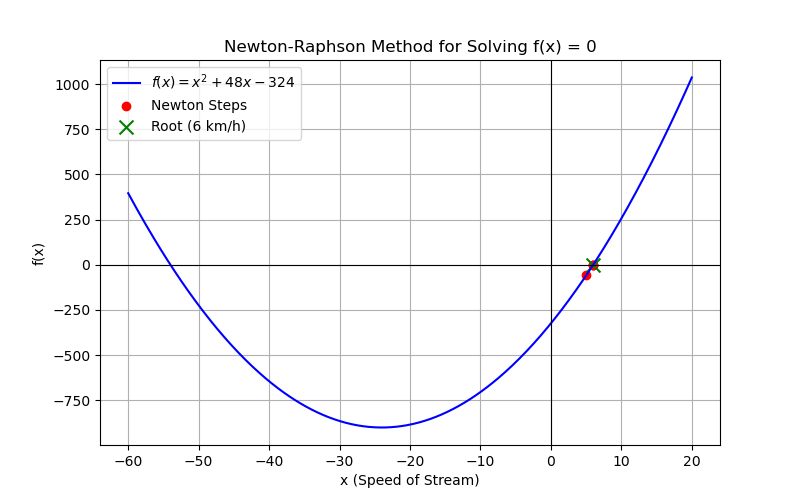
\includegraphics[width=0.8\textwidth]{figures/fig.png} % Ensure this path is correct
   \caption{Plot showing the relationship between $f\brak{x}$ and speed of stream}
   \label{stemplot}
\end{figure}
\end{frame}



\end{document}


